\chapter{Heart rate sensor}\label{ch:heartRate}
%**********************************************

%**********************************************
\section{Introduction} \label{sec:heartIntro}
%**********************************************
Circuits pertaining to signal conditioning, pulse signal and analogue output generation will be discussed. Conditioning is done via filtering and amplification; active filters provide high input and low output impedance, and a large Q-factor \cite{actpas}. A differential amplifier is suitable for amplification, as the gain is referenced against a customizable voltage \cite{opamp}. A Schmitt Trigger is well-suited for pulse generation, as it provides a noise margin \cite{schmitt}. PWM signals can be converted to analogue using filtering \cite{PWM}. 

%**********************************************
\section{Design} \label{sec:heartDesign}
%**********************************************
\begin{figure}[h]
    \centering
    \vspace{-1cm}
    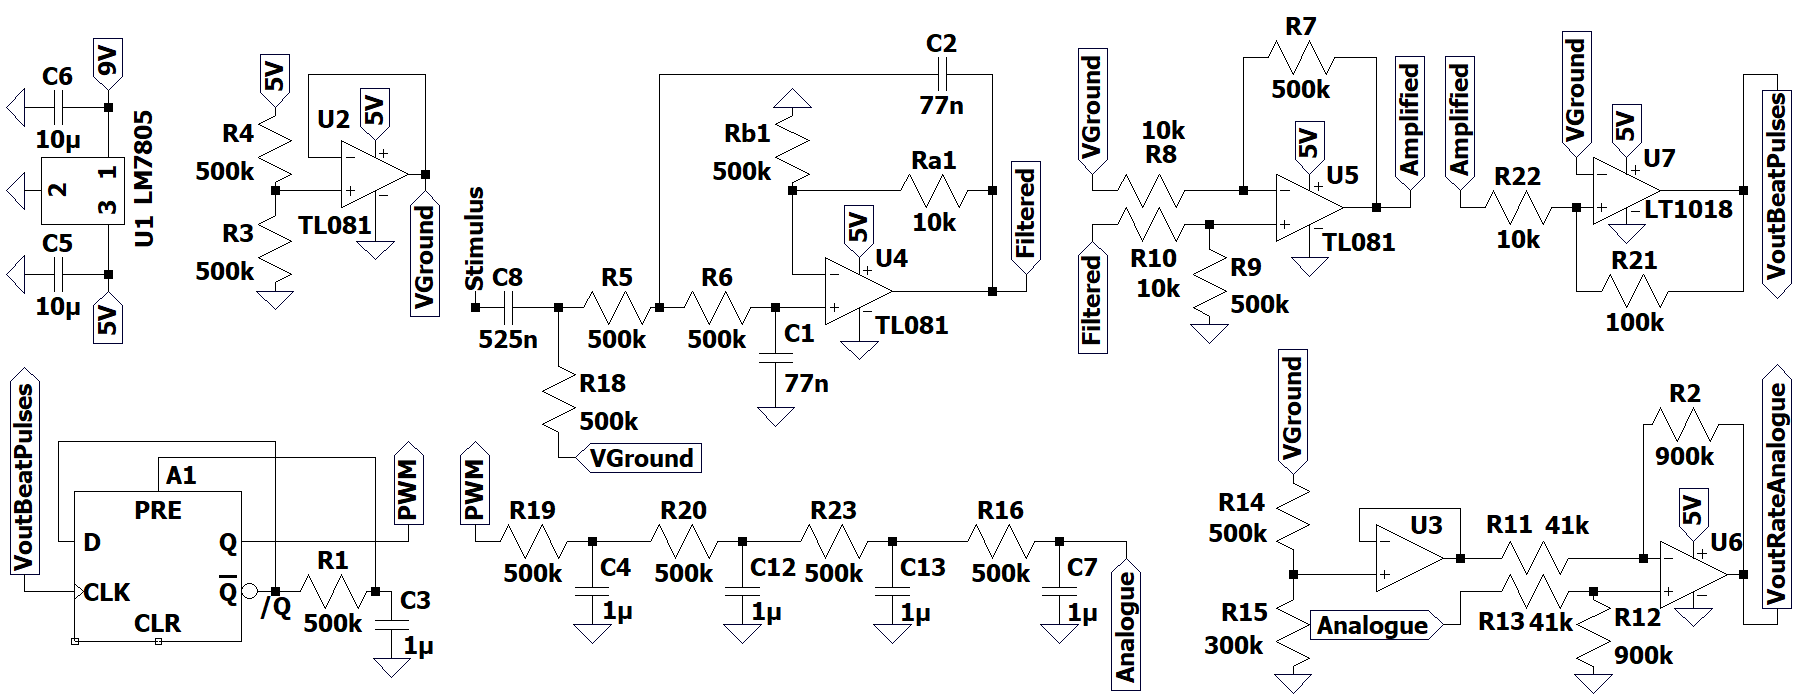
\includegraphics[width = 1\textwidth]{Figures/circuit}
    \caption{Complete Circuit \textbf{enlarge this}}
    \label{fig:circuit}
\end{figure}

\begin{wrapfigure}{r}{0.5\textwidth}
	\vspace{-0.45cm}
    \centering
    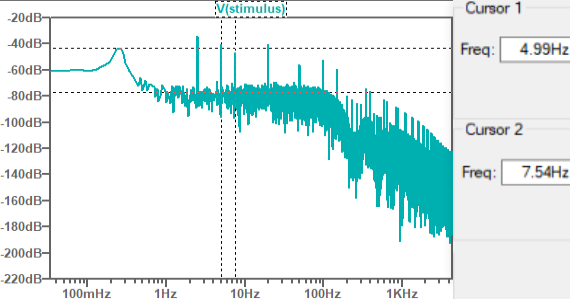
\includegraphics[width = 0.48\textwidth]{./Figures/fft}
    \caption{Fast fourier transform of stimulus}
    \label{fig:fft}
\end{wrapfigure}
The complete circuit is shown upfront in figure \ref{fig:circuit} to aid with explanation. The largest resistor in sub-circuits is always chosen to be \SI{500}{k\Omega}, as to reduce current usage. The design process now follows. The FFT of the stimulus input in figure \ref{fig:fft} has information residing between \numrange{0.8}{2.5} \si{Hz}, corresponding to 50 and 150 BPM respectively. The other peaks represent noise at \SI{0.25}{Hz}, as well as at twice and three times the message signal, and higher. Noise distorts square wave output, necessitating filtering. A first order passive high-pass filter, cutoff frequency \SI{0.606}{Hz}, attenuates the low frequency noise. R18 = \SI{500}{k\Omega}, thus C8 = \SI{525}{nF} according to $f_{c} = \frac{1}{2\pi R C}$. The capacitor is connected to a virtual ground of \SI{2.5}{V}, centering the signal around \SI{2.5}{V}. A second order active low-pass filter, cutoff frequency \SI{4.1}{Hz}, filters out high frequency noise. R5 = R6 = \SI{500}{k\Omega}, C1 = C2 = \SI{77}{nF} - see aforementioned formula. \textbf{mention amplitudes} Cutoff frequencies were selected to remove noise maximally while minimally affecting heart-rate data. The signal should reside slightly above \SI{2.5}{V} to facilitate amplification (to be discussed). Thus, Rb1 = \SI{500}{k\Omega} and Ra1 = \SI{10}{k\Omega} since $A_v=1+\frac{R_{A}}{R_{B}}$ 
\cite{filter}. The TL081 op-amp is used, as it is less expensive than the TLC2272 \cite{octo}. A filter output with DC offset slightly above \SI{2.5}{V} allows for the use of a differential amplifier with the existing virtual ground connected to the negative input, thus removing the need for additional circuitry otherwise required. The signal is amplified according to $\mathrm{V}_{\mathrm{OUT}}=\frac{\mathrm{R}_{a}}{\mathrm{R}_{b}}\left(\mathrm{V}_{2}-\mathrm{V}_{1}\right)$ \cite{opamp}, where R\textsubscript{a} corresponds to R7 and R9, and R\textsubscript{b} to R8 and R10. The gain of 50 was selected to again provide a DC offset of \SI{2.5}{V}, as it facilitates implementation of the comparator (to be discussed). Since the amplified signal has an amplitude of only \SI{1.66}{V}, the inexpensive TL081 was chosen despite having a smaller output range. Next, the signal is fed into a Schmitt Trigger comparator - the LT1018 was chosen as it allows for output very close to 0 and 5V, and has a high gain. \SI{5}{V} is produced if the input exceeds the upper trip point (UTP) and \SI{0}{V} if the input falls below the lower trip point (LTP) \cite{schmitt}. The range between the UTP and LTP is referred to as the hysteresis width ($w_h$) and serves as a noise margin \cite{schmitt} around the reference voltage, $V_{REF_{comparator}}$. The DC offset of \SI{2.5}{V} of the amplified signal requires$V_{REF_{comparator}}$ = \SI{2.5}{V}, once again allowing for the use of the existing virtual ground (instead of additional circuitry) at the negative input of the comparator. Pulse duration is designed for the highest frequency, as it will then also meet the requirement for lower frequencies. Since 150 BPM corresponds to a period of \SI{0.4}{s}, $w_h$ should be selected to ensure an output pulse width of at least \SI{150}{ms}. The amplified signal approximates a sinusoid - substitute values of $t$ that differ by \SI{200}{ms} for $t_1$ and $t_2$ to account for noise:

\begin{equation}
y_1 = 1.66\sin(2\pi(2.5)t_1) + 2.5
\label{eq:sin1}
\end{equation}
\begin{equation}
y_2 = 1.66\sin(2\pi(2.5)t_2) + 2.5
\label{eq:sin2}
\end{equation}

Subtracting \ref{eq:sin2} from \ref{eq:sin1} yields $y_1 - y_2 = w_h =$ \SI{0.52}{V} for $t_1 =$\SI{0.01}{s} and $t_2 =$ \SI{.
21}{s}. $w_h$ also is an order of magnitude larger than the highest input signal noise levels, increasing design fidelity.  Now, UTP = \SI{2.75}{V}, LTP = \SI{2.25}{V}, UTP = $V_{REF} + \beta Vcc$ and LTP = $V_{REF} - \beta Vcc$, thus $\beta$ = 0.05 \cite{schmitt}. Further, $\beta=\frac{\mathrm{R}_{22}}{\mathrm{R}_{22}+\mathrm{R}_{21}}$. Thus R21 = \SI{190}{k\Omega} and R22 = \SI{10}{k\Omega}. (R21 was later adjusted to \SI{100}{k\Omega} to account for loading effects). A one-shot was considered to extend the pulses, but was omitted as the requirement could be met without it. A square wave is thus produced, where the frequency of the pulses represent the heart-rate.\\

Obtaining an output suitable for a microcontroller presents itself as a problem of converting frequency to analogue. The decision was made to obtain a PWM signal from the FM pulse signal, as PWM signals lend themselves more readily to conversion-to-analogue using a simple low-pass RC filter. Pulse-width modulation was achieved by means of a D flip-flop. The essence of the design is to firstly keep the output high continually, but to then drive the output low for a fixed time, once per period. Since the period of the clock signal varies against BPM, driving low for a fixed amount of time results in a different ratio of the pulse being low at different frequencies, producing a varying duty cycle. Specifically, the previously generated pulse signal is used as a clock signal for the D flip-flop, and the not-Q output is fed back into the data line. This would normally drive the output high for all time $t$; thus a RC circuit is added of which the capacitor is charged by the not-Q output, and connected to the SET-line of the flip-flop. Once the capacitor charges to \SI{2.5}{V}, Q is pulled high and not-Q low until the next rising edge of the clock input inverts Q and not-Q. The result is a slightly delayed PWM signal, with a large duty cycle at high frequencies, and vice-versa. This configuration was preferred above the standard one-shot setup, as it results in a consistent PWM output as long as the capacitor charge time is selected to be shorter than the narrowest pulse of the clock signal. See section \ref{sec:heartResults}, figure \ref{fig:pwm} for output graphs.  calculations follow. Selecting R1 = \SI{500}{k\Omega} gives $C = 1\mu$, according to the capacitor charge/discharge exponential equations, of which the extended solution (using a Matlab script) is given in Appendix C for the sake of brevity. Having obtained a PWM signal, a fourth order passive low-pass filter produces analogue values in the range of \numrange{0.95}{1.2} \si{V}. A cutoff frequency of \SI{0.5}{Hz} ensures maximal attenuation of noise while maintaining a 5\% settling time of 10 seconds. Therefore resistor values are \SI{500}{k\Omega} and capacitor values are \SI{1}{\mu}. Finally, the analogue output is amplified by means of a differential amplifier, using a TLC2272, with a negative input at \SI{0.938}{V}. A gain of 20 produces a sufficient output range. Resistor values were chosen to be larger as to minimize loading effects. Thus, R2 = R12 = \SI{900}{k\Omega} and R11 = R13 = \SI{45}{k\Omega} according to $\mathrm{V}_{\mathrm{OUT}}=\frac{\mathrm{R}_{a}}{\mathrm{R}_{b}}\left(\mathrm{V}_{2}-\mathrm{V}_{1}\right)$ \cite{opamp}. Loading effects still had a slight effect, and required adapting R11 and R13 to \SI{41}{k\Omega}. An analogue transducer is thus designed, and can be connected to a microcontroller.

Total current is calculated using \SI{1.4}{mA} per TL081 \cite{tl081}, \SI{2.2}{mA} per TLC2272 \cite{tlc2272} and \SI{110}{\mu A} per LT1018 \cite{lt1018}. Non-trivial resistors are all approximated using \SI{5}{V} over, as to err on the side of caution: $4(1.4m) + (2.2m) + (110n) + 16\left(\frac{5}{500k}\right) + 3\left(\frac{5}{10k}\right) +
 2\left(\frac{5}{41k}\right) + \left(\frac{5}{100k}\right) =$ \SI{9.75}{mA}. Voltage regulator current is considered in E344 Assignment 1 \cite{prev}. $100m - 9.75m - 11.39m$ leaves \SI{78.86}{mA} for Assignment 3.

%**********************************************
\section{Results} \label{sec:heartResults}
%**********************************************
The frequency response of both the high- and low-pass filters are $-3dB$ at \SI{0.606}{Hz} and $-6dB$ at \SI{4.3}{Hz} respectively, as shown in figures \ref{subfig:hpf} and \ref{subfig:lpf1}, thus matching the design calculations almost perfectly. Comparison of filter input and output in figure \ref{fig:filtout} shows a drastic reduction in noise. 

\begin{figure}[h]
 \footnotesize
   \centering
   \begin{subfigure}[]{0.48\textwidth}
        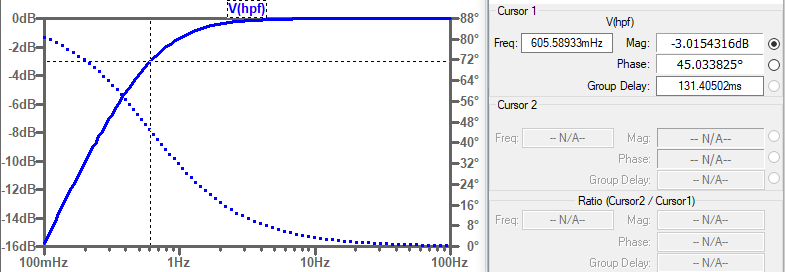
\includegraphics[width=\linewidth]{./Figures/hpf}
	  \caption{High-pass filter} \label{subfig:hpf}	
   \end{subfigure}
   \begin{subfigure}[]{0.48\textwidth}
  	 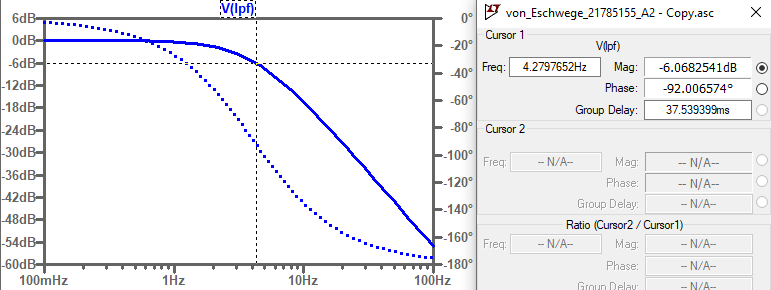
\includegraphics[width=\linewidth]{./Figures/lpf1}
	  \caption{Second-order low-pass filter} \label{subfig:lpf1}	
   \end{subfigure}
   \caption {Frequency response of filters}.
   \label{fig:freqreq}
 \end{figure}
  
\begin{wrapfigure}{l}{0.3\textwidth}
\centering
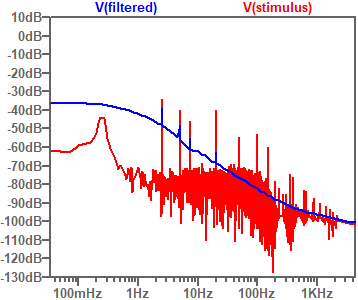
\includegraphics[width=0.3\textwidth]{./Figures/filtout}
\caption{Filter input and output}
\label{fig:filtout}
\end{wrapfigure}

The filtered signal is passed through a differential amplifier; the input is shown in blue and the output in red in figure \ref{fig:amplified}. The filtered signal has a \SI{50}{mV} amplitude (peak-to-peak), and the output \SI{1.747}{V}. Therefore $A_v \approx 35$, which, although smaller than calculated, is to be expected due to non-linear behaviour for high amplification factors. 

\begin{figure}[h]
 \footnotesize
   \centering
   \begin{subfigure}[]{0.49\textwidth}
        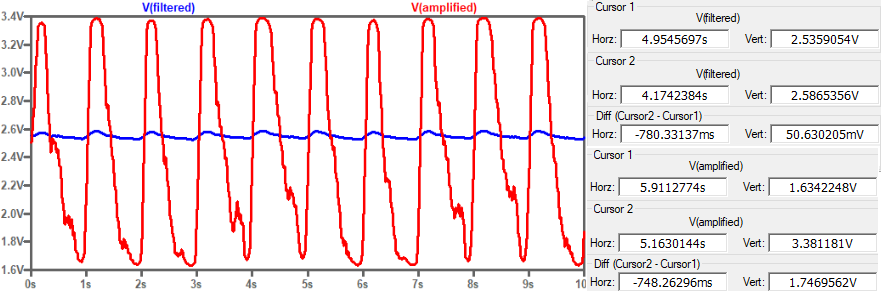
\includegraphics[width=\linewidth]{./Figures/amplified}
	  \caption{Amplification of filtered signal} \label{subfig:amplified}	
   \end{subfigure}
   \begin{subfigure}[]{0.49\textwidth}
  	 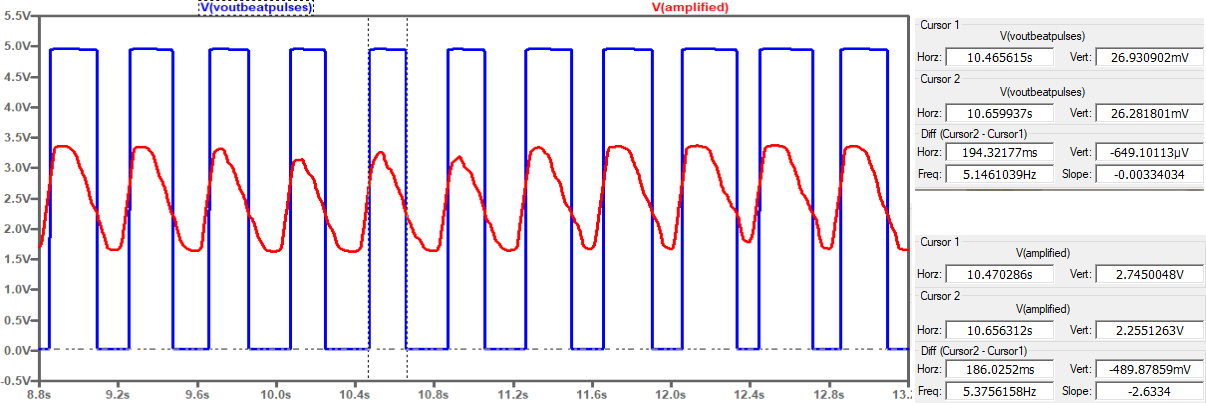
\includegraphics[width=\linewidth]{./Figures/pulses}
	  \caption{Thresholding} \label{subfig:pulses}	
   \end{subfigure}
   \caption{Signal Conditioning}
 \end{figure}

Input and output of a LT1018 comparator, used for thresholding, is shown in figure \ref{fig:pulses}.  See UTP = \SI{2.75}{V} and LTP = {2.25}{V} in figure \ref{fig:pulses}, giving a hysteresis width of \SI{0.5}{V}, exactly as calculated. The output ranges from \numrange{0.026}{4.95}\si{V}, with a pulse duration in range \numrange{189}{584} \si{ms} in figures \ref{subfig:pulses2} and \ref{subfig:pulses1}, meeting the \SI{150}{ms} requirement. The design remains consistent for specification deviations of $\pm 10\%$ amplitude and a DC offset variation of $\pm$ \SI{0.2}{V}, as the high-pass filter removes the DC component and the filter has a cutoff frequency low enough to greatly attenuate noise.

\begin{figure}[h]
 \footnotesize
   \centering
   \begin{subfigure}[]{0.49\textwidth} 	 
  	 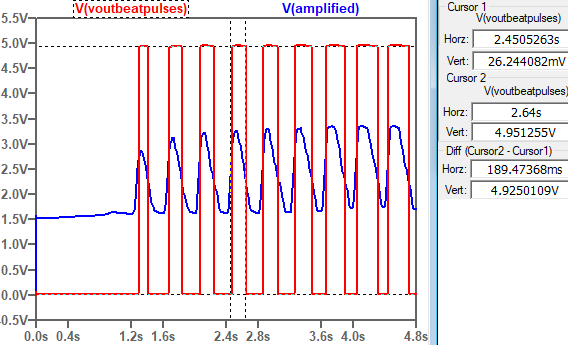
\includegraphics[width=\linewidth]{./Figures/pulses2}
	  \caption{150 BPM} 
	  \label{subfig:pulses2}	
   \end{subfigure}
   \begin{subfigure}[]{0.49\textwidth}
        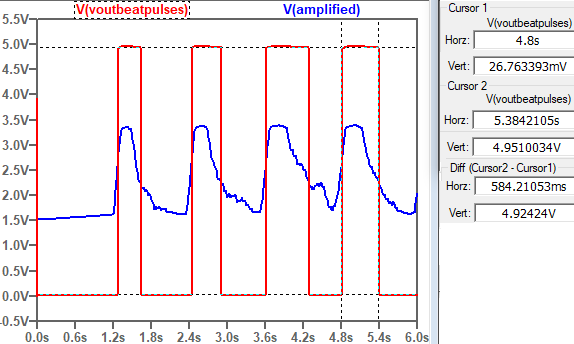
\includegraphics[width=\linewidth]{./Figures/pulses1}
	  \caption{50 BPM} 
	  \label{subfig:pulses1}	
   \end{subfigure}
 \end{figure}

For the analogue transducer, a PWM signal is obtained. Section \ref{sec:heartDesign} explains the interrelation of the signals, where \texttt{voutbeatpulses, pwm} and \texttt{rc} in figure \ref{fig:pwm} correspond to the clock signal, Q, and the charging capacitor voltage respectively. The 5\% settling time is \SI{9.45}{s}. The duty cycle is 73\% at 60 BPM and decreases to 56\% at 150 BPM. Finally, amplification and filtering of the PWM signal produces analogue output, range \SI{4.2}{V} (\ref{subfig:analog}).

\begin{figure}[h]
 \footnotesize
   \centering
   \begin{subfigure}[]{0.57\textwidth}
        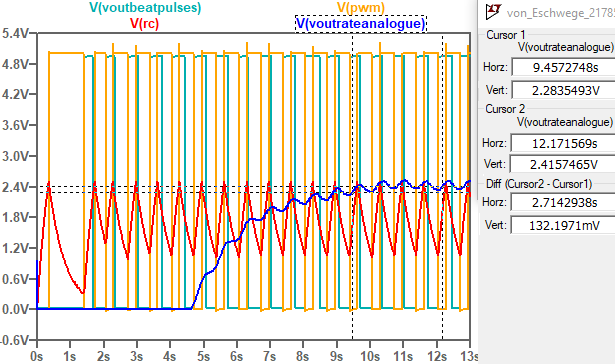
\includegraphics[width=\linewidth]{./Figures/pwm}
	  \caption{PWM and settling time} 
	  \label{subfig:pwm}	
   \end{subfigure}
   \begin{subfigure}[]{0.41\textwidth}
  	 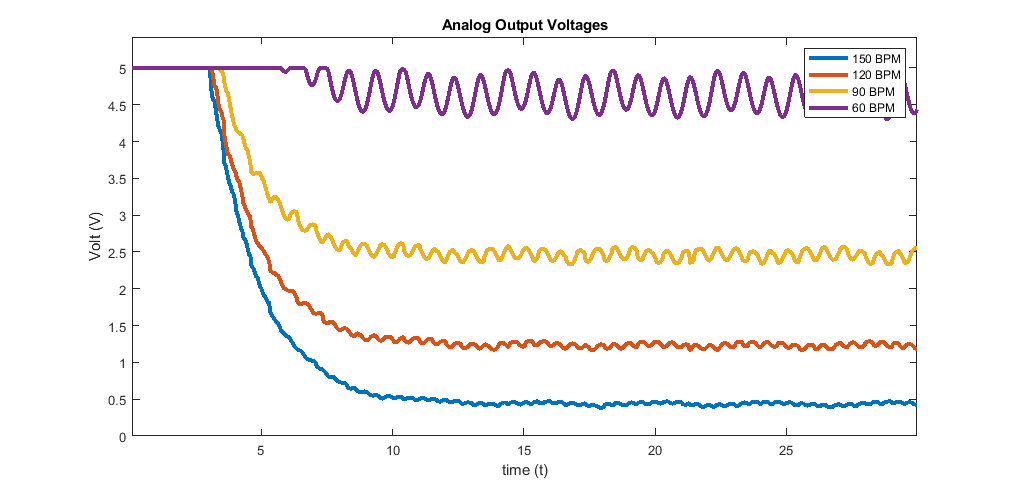
\includegraphics[width=\linewidth]{./Figures/analog}
	  \caption{Analogue voltage output} 
	  \label{subfig:analog}	
   \end{subfigure}
 \end{figure}
 
In figure \ref{fig:current}, total current draw is measured through R\textsubscript{sense}, averaging \SI{12.9}{mA}, meeting the bonus requirement of \SI{15}{mA}. When combined with Assignment 1, the combined current of \SI{25.8}{mA} still is far less than the maximum current rating of \SI{100}{mA} for the voltage regulator \cite{prev}. 

 \begin{wrapfigure}{r}{0.4\textwidth}
\centering
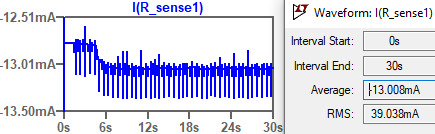
\includegraphics[width=0.4\textwidth]{./Figures/current}
\caption{Total current usage}
\label{fig:current}
\end{wrapfigure}

%**********************************************
\section{Summary}\label{sec:temp_summary}
%**********************************************
Concluding, it has been shown that the design performs as expected, meeting the all requirements. Output pulse width is broader than required, analogue output is generated with discrete, non-overlapping values exceeding the required range, while settling to a final value according to specification.  Current draw remains sub-\SI{15}{mA}. Upon implementation of the microcontroller, be cognizant of the fact that analogue output values scale in a slightly non-linear fashion. This is not a problem, as it can be easily accounted for in software.

